\section{Initial Ideas}
The duck's name is encoded as ASCII characters and framed as UART packets in an ultrasonic signal.
\begin{figure}[h]
    \centering
    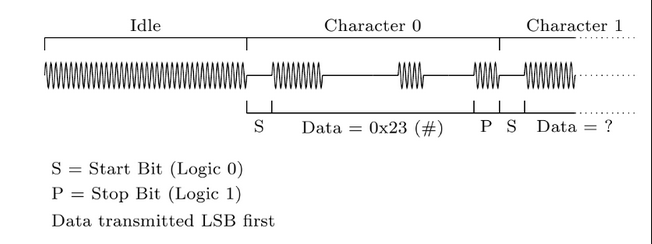
\includegraphics[width=0.8\textwidth]{subpages/images/ultra_spec.png}
    \caption{Model for the Output of the Duck's Name [2]}
    \label{fig:ultrasound_specifications}
\end{figure}

The communication works as such:
\begin{itemize}
    \item The start bit, S, indicates the start of an ASCII character
    \item The next bits will then produce a character, to indicate the letter. This can be seen in character 0 where the data is equal to 0x23, this is hexadecimal for the ASCII character `\#'.
    \item The last bit, P, is the stop bit indicating the end of an ASCII character (Note that each duck's name will start with the `\#').
\end{itemize}

To obtain these bits, an ultrasound transducer is used to pick up the ultrasound signal of the duck. This signal is then demodulated and converted to a binary signal using a comparator. The output from the comparator is connected to the microcontroller which has UART communication built in decoding the binary signal into bytes.

The overall circuit shown below can be split into 3 stages: the ultrasound signal (and amplification); the envelope detector; and the comparator circuit via a Schmitt trigger. These combine to give the desired bitwise logic shown in figure 5.2.
\begin{figure}[h]
    \centering
    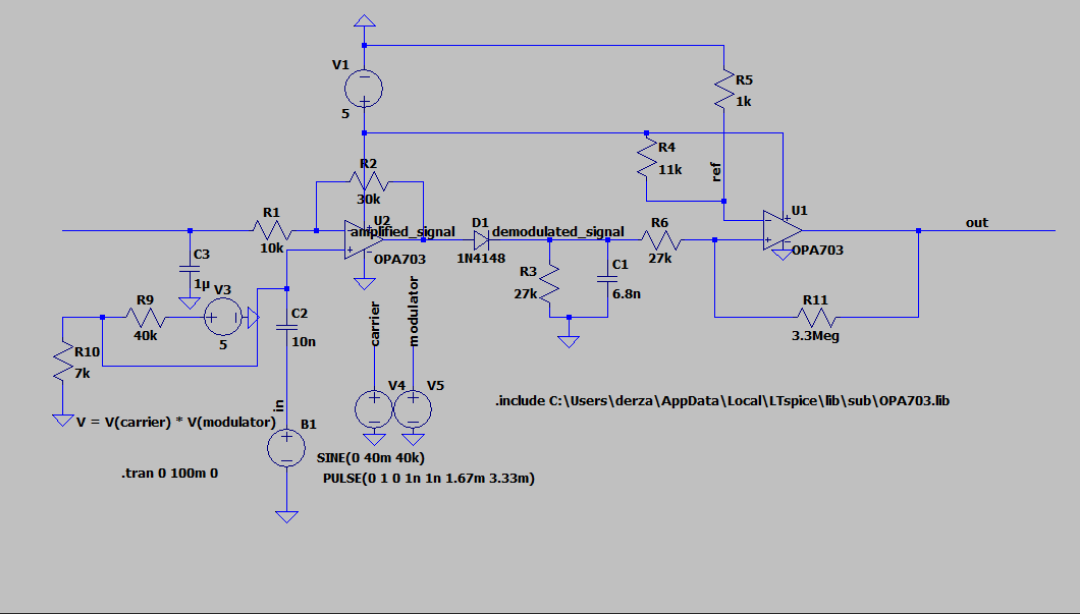
\includegraphics[width=0.8\textwidth]{subpages/images/ultra_circuit_naming.png}
    \caption{LTspice Circuit Diagram for the Duck Naming Process}
    \label{fig:ultrasound_naming_circuit}
\end{figure}

\section{The Ultrasound Signal}
The ducks communicate using a carrier frequency of 40kHz modulated with a form of amplitude-shift-keying (ASK), where an amplitude of 0 represents logic 0 and an amplitude much greater than 0 represents logic 1.

A piezoelectric transducer was used as it operates around the required level and can effectively convert mechanical vibrations into electrical signals [3]. Moreover, as they have a high range of frequencies, i.e. they can measure a large range, they are the most ideal transducers.

The MCUSD16A40S12RO [4] transducer was selected due to its high sensitivity as well as being compact and lightweight. Moreover, it has a low power consumption, which is a benefactor for our high efficiency target.
\begin{figure}[h]
    \centering
    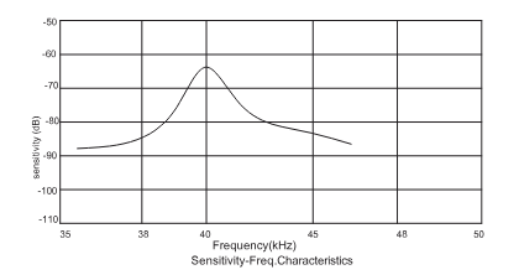
\includegraphics[width=0.8\textwidth]{subpages/images/ultra_sensitive_freq.png}
    \caption{Sensitivity-Frequency Graph for MCUSD16A40S12RO}
    \label{fig:sensitivity_frequency}
\end{figure}

This transducer was tested practically, giving the signal shown below.
\begin{figure}[h]
    \centering
    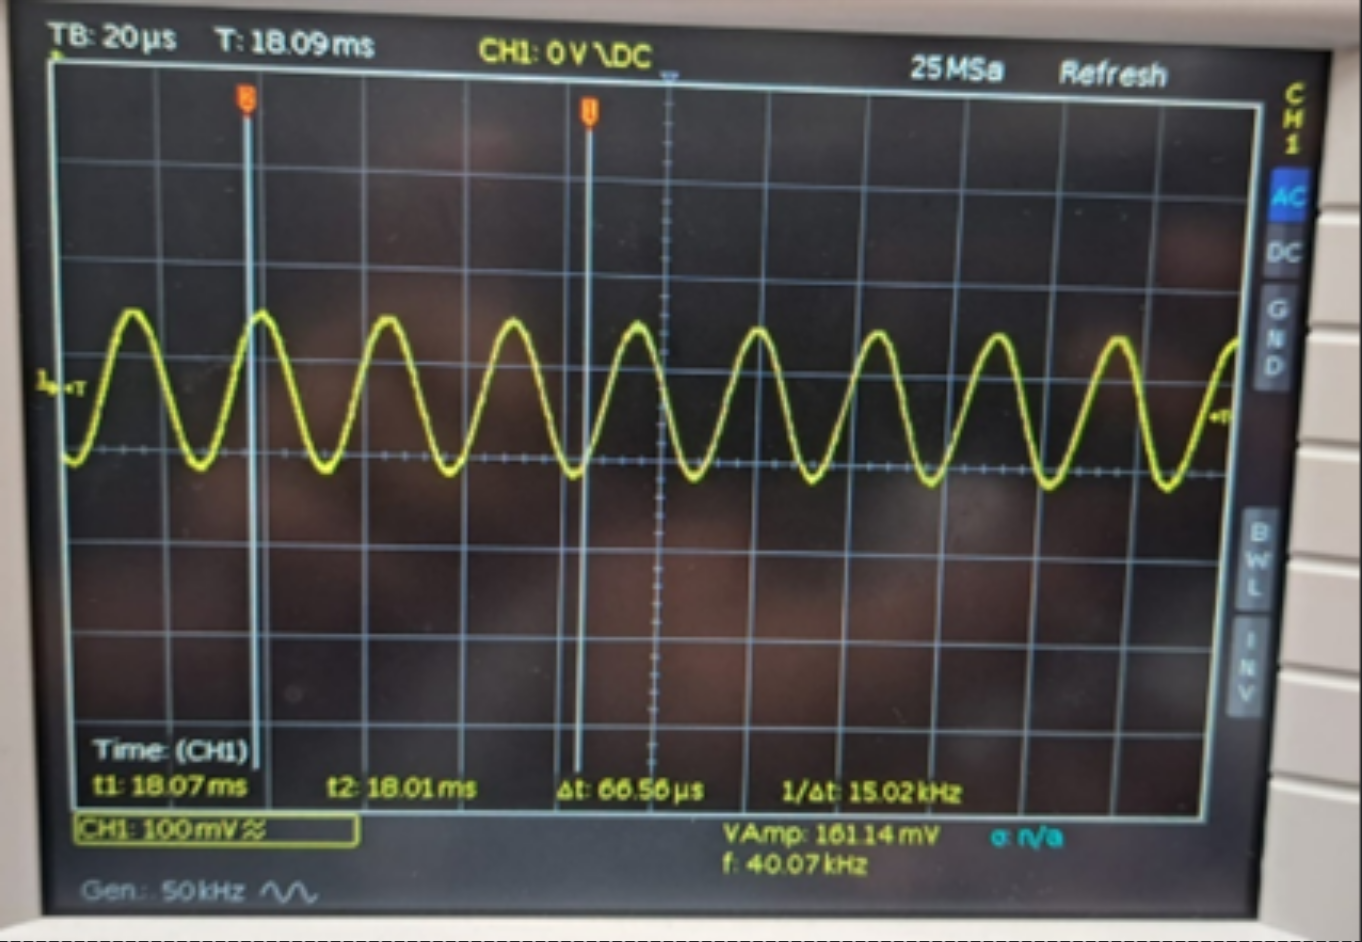
\includegraphics[width=0.8\textwidth]{subpages/images/ultra_oscilloscope_transducer.png}
    \caption{Oscilloscope Waveform of Transducer Signal at Around 160mV Amplitude}
    \label{fig:transducer_waveform}
\end{figure}
To model the sinusoidal waves generated by the sensor, the first section of the overall circuit has been shown below:
\begin{figure}[H]
    \centering
    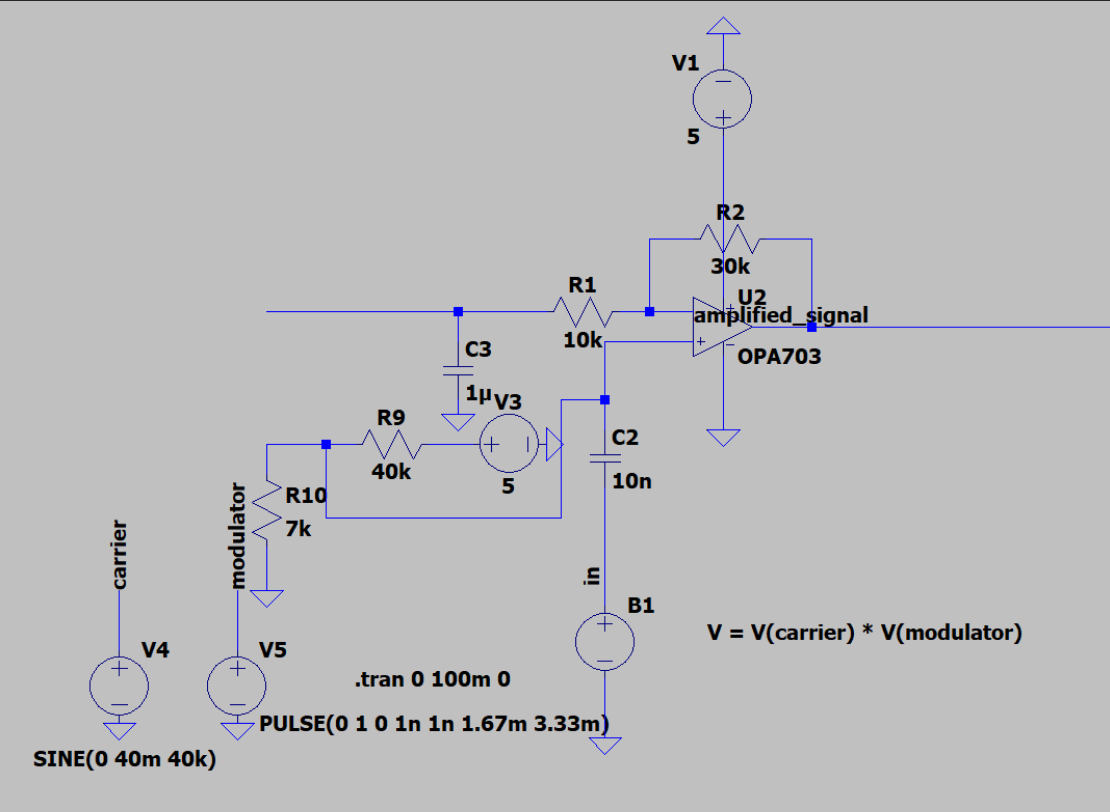
\includegraphics[width=0.8\textwidth]{subpages/images/ultra_circuit_trans_amp.png}
    \caption{Circuit Schematic for the Ultrasound Transducer and Amplifier}
    \label{fig:transducer_amplifier_circuit}
\end{figure}
The behavioural voltage source, B1, is defined by the product of the carrier signal, a sine wave with a frequency of 40kHz and amplitude of 40mV, and a modulated signal, imitating the ASK modulation stated prior. Given a transient simulation running for 100ms on LTspice, the waveform produced the expected output. It should be noted that a 40mV amplitude was used in simulation as an estimate of the amplitude from the transducer.

\begin{figure}[h]
    \centering
    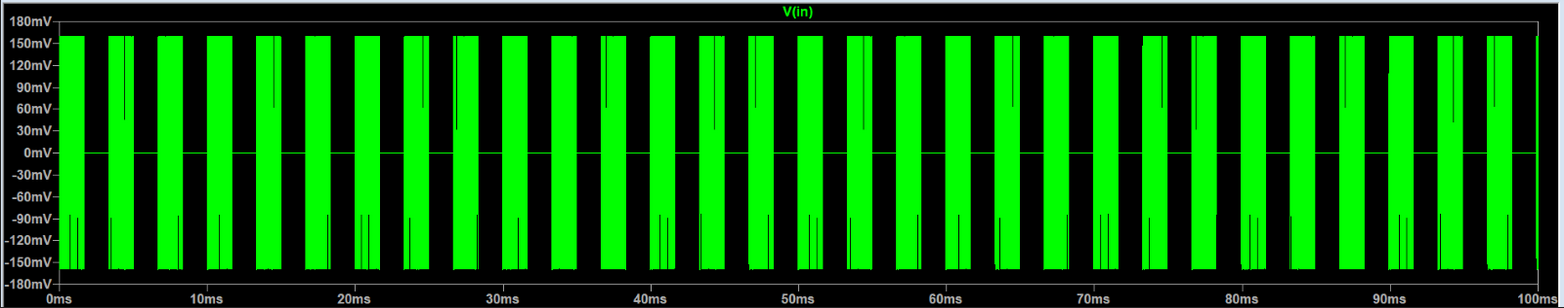
\includegraphics[width=0.8\textwidth]{subpages/images/ultra_bv_output.png}
    \caption{Output Waveform for the Behavioural Voltage Source}
    \label{fig:bv_waveform}
\end{figure}
The amplitude of this signal shown in LTspice is 150mV, this signal is extremely low and thus requires amplification to allow for envelope detection and to act as a binary signal. A large voltage difference is required between the high and low outputs, this cannot be achieved with a 150mV input to a comparator. Therefore, this signal must be amplified. This is done using a non-inverting amplifier.  The non-inverting amplifier was chosen due to having a positive gain as well as having a simple design (Cadence PCB Solutions, 2024).
\begin{figure}[h]
    \centering
    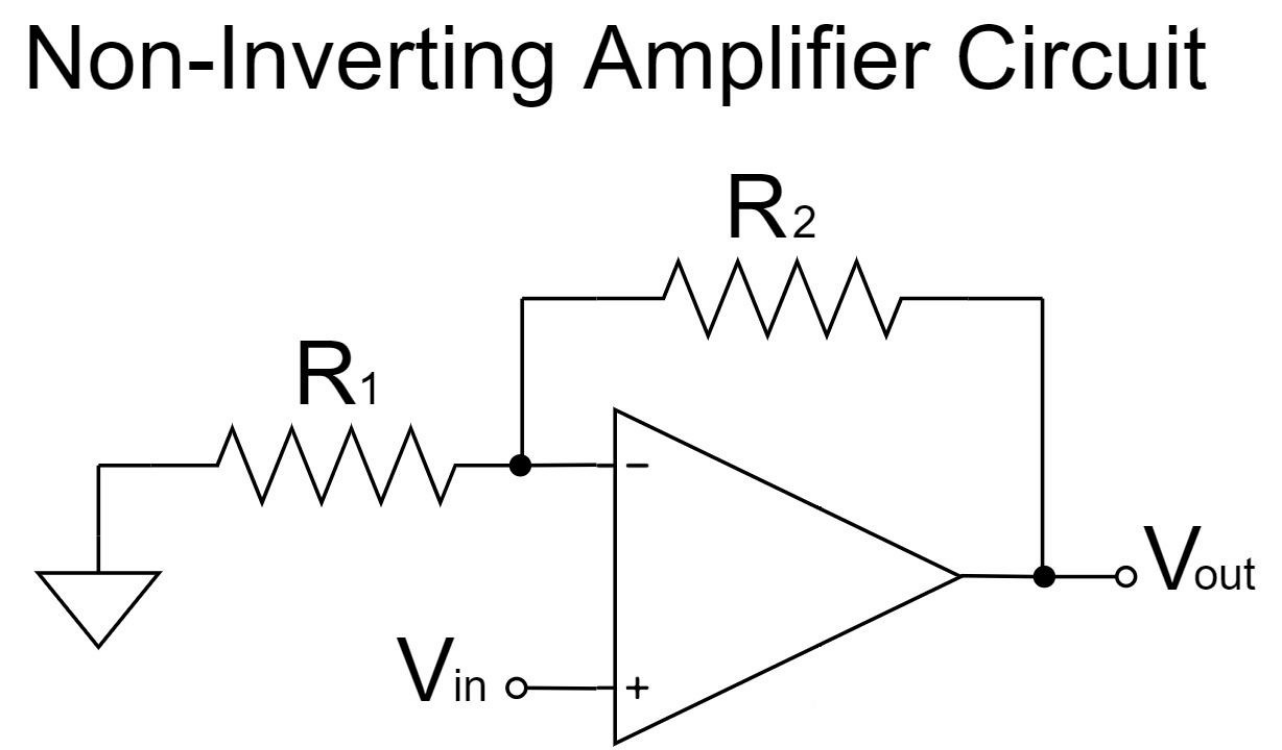
\includegraphics[width=0.8\textwidth]{subpages/images/non_invert_amp.png}
    \caption{Non-Inverting Amplifier Circuit (Spiceman, 2022)}
    \label{fig:non_inverting_amp}
\end{figure}
Given this circuit, the gain of the circuit is given as such: \(1+ \frac{R_f}{R_{In}} \).

A gain of 4 was deemed to give a high enough output to allow for the next stages of the circuit to work effectively. This is achieved with R2 being equal to 30k and R1 being 10k. This produces the desired output shown below. Furthermore, due to the bias signal connected to the non-inverting input of the op-amp, the DC offset is around 750mV, this is much lower when practically built which will be important in the next stage of the circuit.  A key point is that there is no ground in the negative input of the amplifier, ensuring there is no DC offset from it.
\begin{figure}[h]
    \centering
    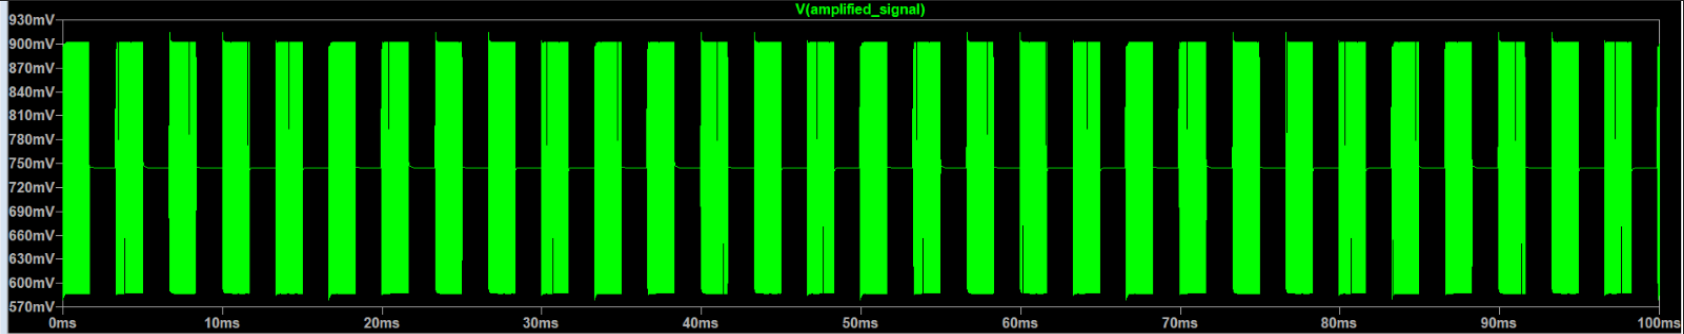
\includegraphics[width=0.8\textwidth]{subpages/images/ultra_output_amplified.png}
    \caption{Output Waveform for the Amplified Signal}
    \label{fig:amplified_output}
\end{figure}

Researching components suggests that an array of op-amps will be required in this project rather than mimicking op-amps from previous sections for the sake of simplicity. In this case, the OPA703 op-amp was used due to its high slew rate of 0.6V/µs, thus allowing for a quick response to the change in signals [5]. Moreover, it allowed for a rail-to-rail input/output thus allowing for the power rails to be 5V and 0V. This also allows for the output waveform to stay positive due to the ground-referenced supply to the negative power rail of the op-amp.

Building further, the low quiescent current of 160µA makes this op-amp suitable for relatively low-power applications such as a duck detection system as the electronic architecture of the work is not overly power-demanding. With an input voltage noise density of \(45nV/\quad{Hz}\) and low offset voltage, the OPA703 limits noise interference, which is crucial for detecting small-amplitude signals from the transducer. Therefore, this greatly enhances the signal-to-noise ratio during amplification. The additional presence of high common-mode rejection ratio of 90dB ensures that common-mode noise is rejected.
\begin{figure}[h]
    \centering
    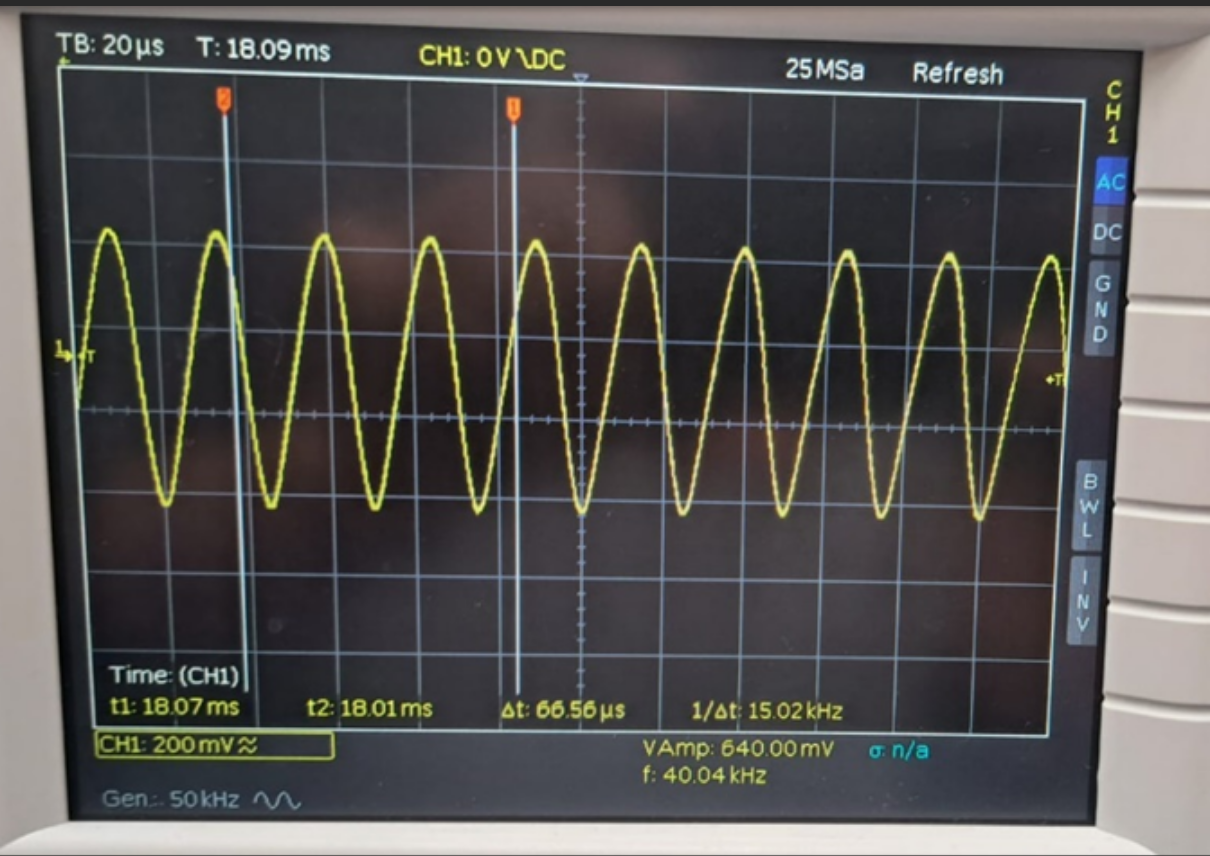
\includegraphics[width=0.8\textwidth]{subpages/images/ultra_4_gain.png}
    \caption{Waveform of 4x Amplified Ultrasonic Signal}
    \label{fig:waveform_4x_gain}
\end{figure}

\section{Envelope detector}
The envelope detector demodulates the signal from the ultrasound transducer, involving the extraction of a desired signal from a modulated carrier signal at the receiver end.
\begin{figure}[h]
    \centering
    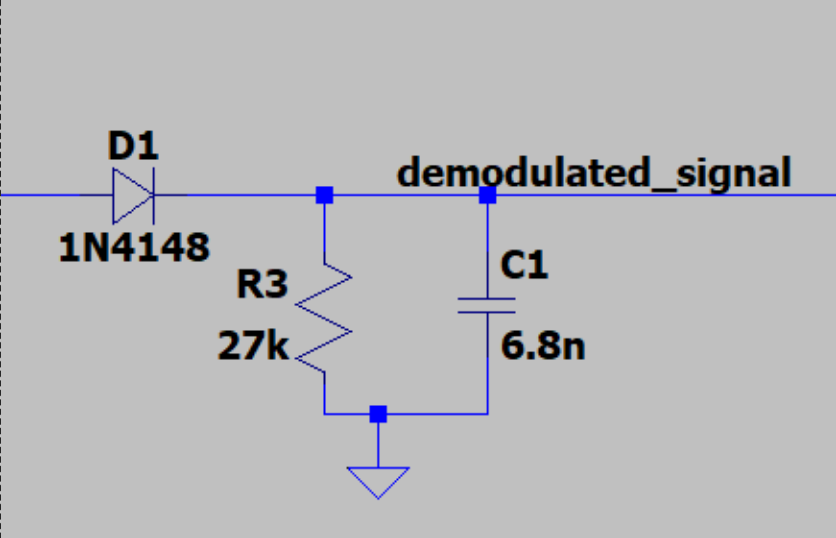
\includegraphics[width=0.8\textwidth]{subpages/images/ultra_envelope.png}
    \caption{Circuit Schematic for the Envelope Detector}
    \label{fig:envelope_detector}
\end{figure}
The diode is used to reduce the amplitude of oscillations due to the op-amp thus demodulating the signal [6]. The diode chosen was the 1N4148 for its fast-switching and cheap price7. In the section prior, it was mentioned that a low DC offset was key for the next section. This is because due to the ASK modulation, when a low input was given, a high DC offset would cause the diode to remain on and thus there would be no change in a logic 1 and 0 input in the final output. The expected output can be seen in the figure below:
\begin{figure}[h]
    \centering
    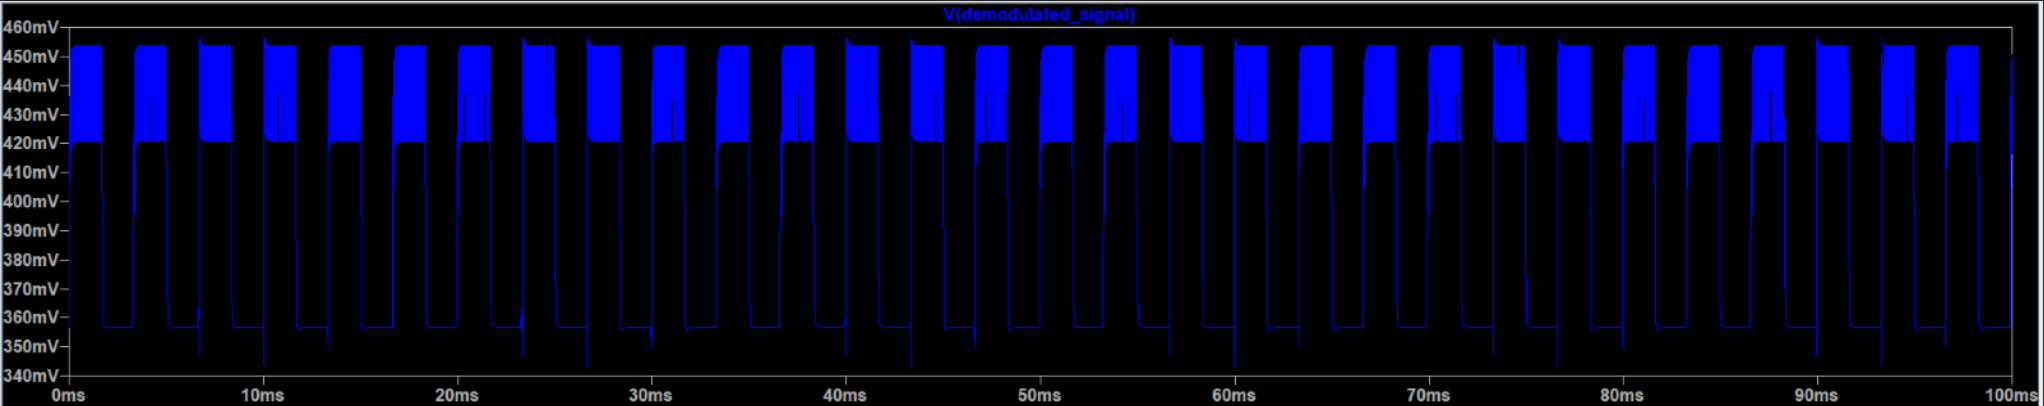
\includegraphics[width=0.8\textwidth]{subpages/images/ultra_output_demodulated.png}
    \caption{Output Waveform for the Demodulated Signal}
    \label{fig:demodulated_waveform}
\end{figure}

The low pass filter after the diode is used to ensure that the carrier frequency is filtered out. Moreover, as the signals of the duck have a frequency of 600Hz, given by the 600 bits per second stated in the introduction, this frequency must be passed through the filter. Therefore, the corner frequency of this filter must be significantly under 40kHz and greater than 600Hz to ensure that all required signals are picked up accounting for any fluctuations from the stated frequencies. Therefore, the corner frequency was chosen to be 900Hz. The equation used: \(f_c = \frac{1}{2\pi RC}\)

Given that: RC must be equal to approximately 0.184ms; and the available components in the lab, the following values of R and C in figure 29 were chosen. This gave a corner frequency of 867Hz shown to be achieved through AC analysis on LTspice.
\begin{figure}[H]
    \centering
    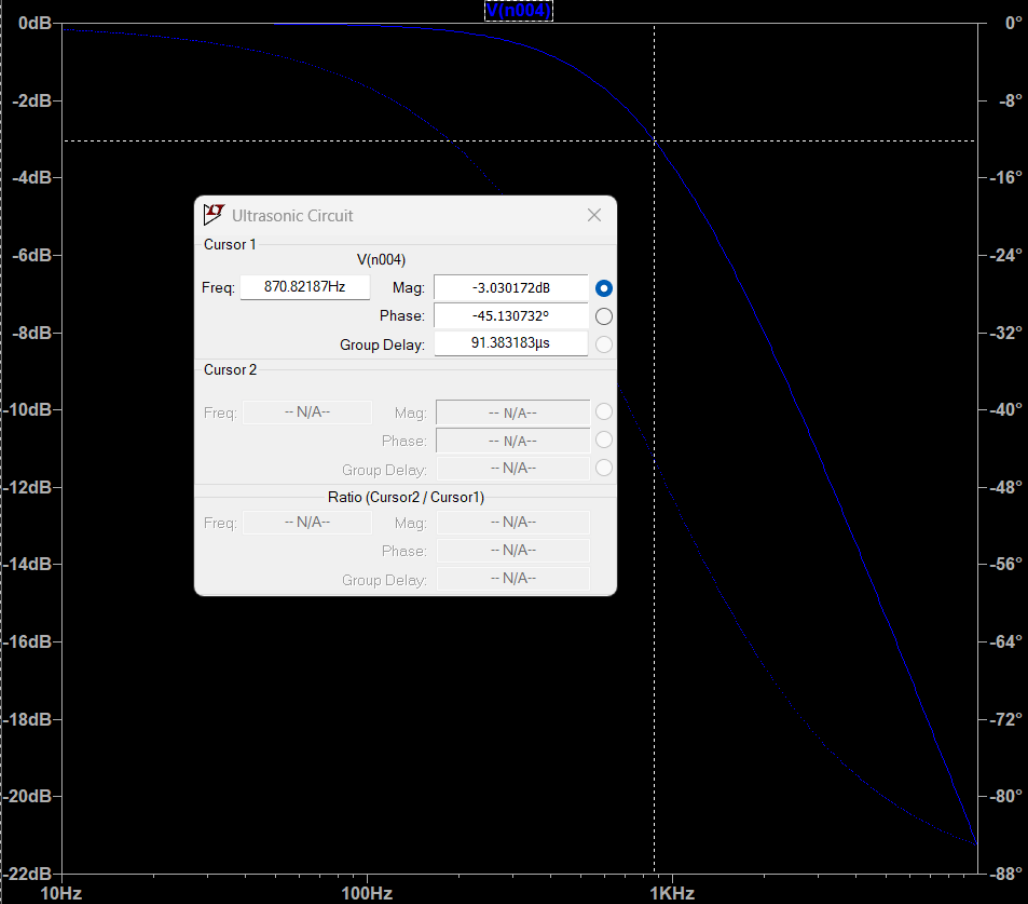
\includegraphics[width=0.45\textwidth]{subpages/images/ultra_lp.png}
    \caption{Magnitude Response for the Low-Pass Filter With its Corner Frequency}
    \label{fig:mag_response_lp}
\end{figure}

\section{Comparator}
A Schmitt trigger is used as a comparator to convert the demodulated analogue signal from the envelope detector to a digital signal by giving a high output when the voltage reaches a certain threshold and giving an output of zero volts otherwise [8].
\begin{figure}[h]
    \centering
    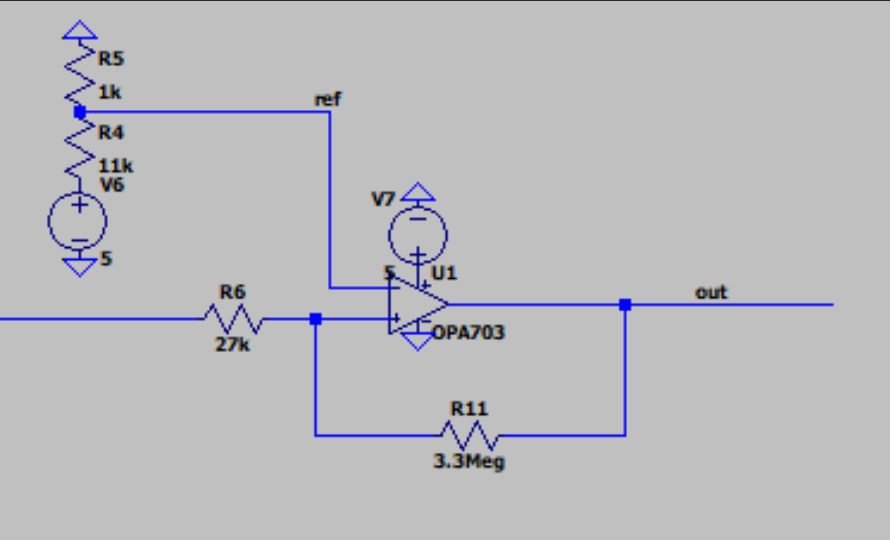
\includegraphics[width=0.8\textwidth]{subpages/images/ultra_comparator.png}
    \caption{Circuit Schematic for the Comparator Circuit}
    \label{fig:comparator}
\end{figure}

The voltage divider is given by the V6, R4 and R5. This provides the reference voltage for the comparator connected at V-. The reference voltage, Vref, is given as such: \(V_{ref}  = \frac{R_5}{R_5 + R_6}V_{CC}\)

Given Vcc = 5V, the resister values in figure 32 were chosen as they gave the most accurate signals as well as the sharpest transitions between the high and low states; a high resistance for R4 would cause a slower transition and a lower resistance would cause chattering, multiple rapid transitions [9], in the output. This gives the reference voltage of 412mV shown below.
A Schmitt trigger is used as a comparator to convert the demodulated analogue signal from the envelope detector to a digital signal by giving a high output when the voltage reaches a certain threshold and giving an output of zero volts otherwise [8].
\begin{figure}[h]
    \centering
    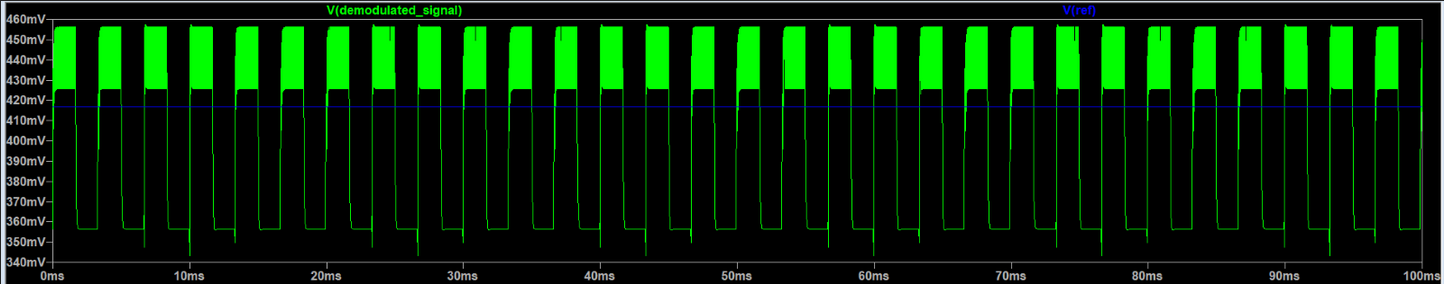
\includegraphics[width=0.8\textwidth]{subpages/images/ultra_reference_out.png}
    \caption{Output Waveform for the Reference Voltage Relative to the Demodulated Signal}
    \label{fig:reference_output}
\end{figure}

Originally, an MP6561 output comparator was going to be used [10], however due to these comparators being surface mount components exclusively, this comparator was not suitable due to issues with prototyping and other sections required for the overall project11 i.e. it would make it more difficult to implement with the entire rover.

Therefore, the OPA703 op-amp is used here to function as a comparator. Although it has a slower slew rate than the MP6561, this should not be an issue due to the slow input transitions compared to this rate. As an op-amp is used rather than a comparator, the Schmitt trigger is used to reduce chattering when built practically. This is because there is greater hysteresis in this design in comparison to using a comparator circuit.
\begin{figure}[h]
    \centering
    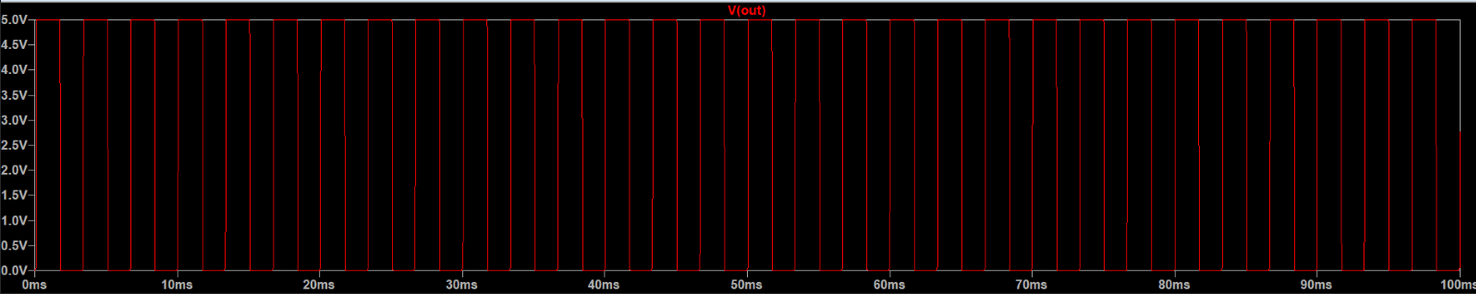
\includegraphics[width=0.8\textwidth]{subpages/images/ultra_binary_out.png}
    \caption{Output Waveform of the Binary Signal}
    \label{fig:binary_signal}
\end{figure}
\begin{figure}[h]
    \centering
    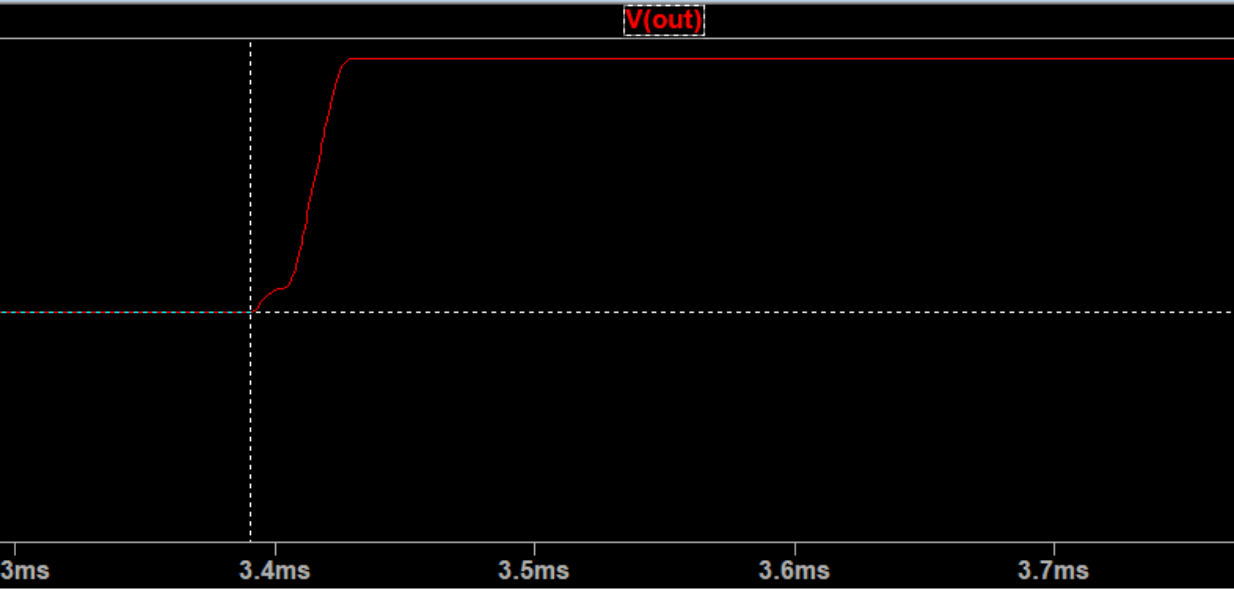
\includegraphics[width=0.8\textwidth]{subpages/images/ultra_binary_transition.png}
    \caption{Output Waveform of the Binary Signal at the Transition. The transition Time via LTspice was 37$\mu$s}
    \label{fig:binary_transition}
\end{figure}

The overall circuit was then constructed and assessed to give binary outputs.
\begin{figure}[H]
    \centering
    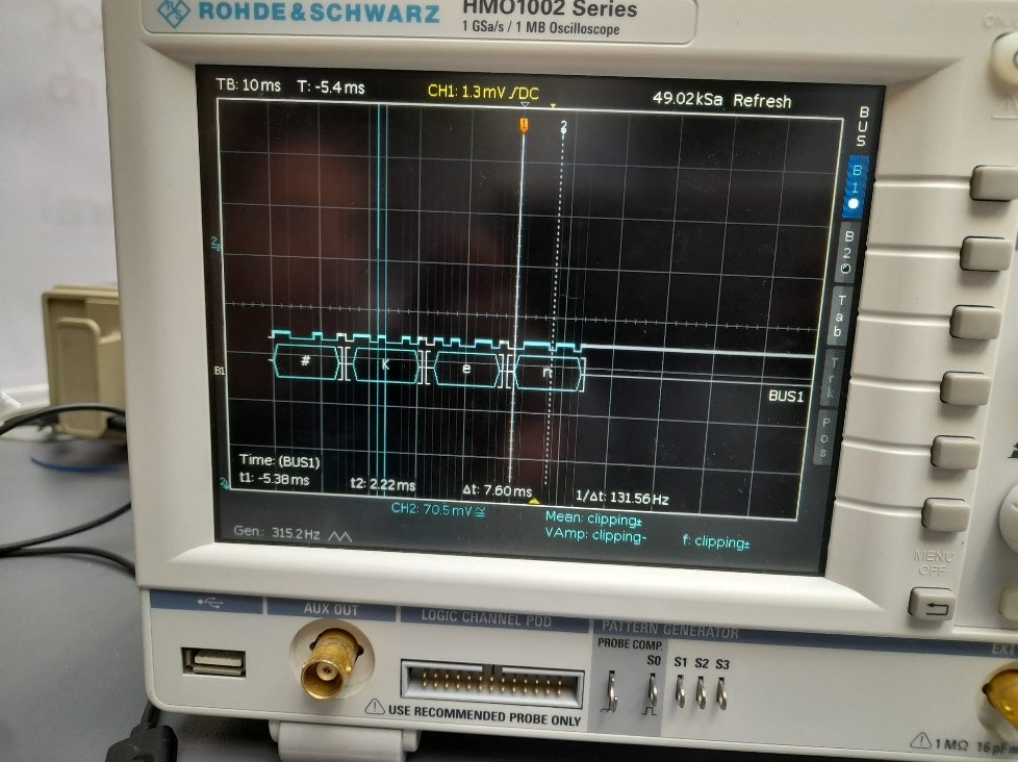
\includegraphics[width=0.6\textwidth]{subpages/images/ultra_out.png}
    \caption{Oscilloscope Waveform of the Output Binary Signal}
    \label{fig:binary_transition}
\end{figure}
In conclusion, the ultrasonic detection circuit produces the binary output shown in figure 5.17. Future improvements to this design may include higher gain in the amplifier circuit allowing for detection at a further distance and increased hysteresis in the comparator reducing the chattering in the final output. A key concept in building this circuit was demodulation. This continued to be integral in signal analyses as seen in the construction of the radio detectors.